% =============================================================================
% SEÇÃO 3.3: IMPACTO FINANCEIRO GLOBAL E BREAK-EVEN (PESSOA 3 — JOÃO)
% Formato Condensado: 2 Páginas ACM sigconf
% =============================================================================

\subsection{Global Financial Impact \& Break-Even Dynamics}
\label{sec:financial_impact}

Commercial LLM APIs bill on a strict per-token basis~\cite{ahia2023all,openai2024gpt4o}. We simulate a production workload of $N = 10^6$ requests (prompt $+$ completion of 300 words $\approx 15$ parallel FLORES-200 sentences~\cite{goyal2022flores}), weighting languages by empirical web traffic (W3Techs~\cite{w3techs2024languages}) under blended pricing for OpenAI GPT-4o (\$4.38/1M tokens)~\cite{openai2024gpt4o}, Claude 3.5 (\$6.00/1M)~\cite{anthropic2024claude}, and Llama 3.1 70B (\$0.80/1M)~\cite{meta2024llama3}.

\begin{figure}[t]
    \centering
    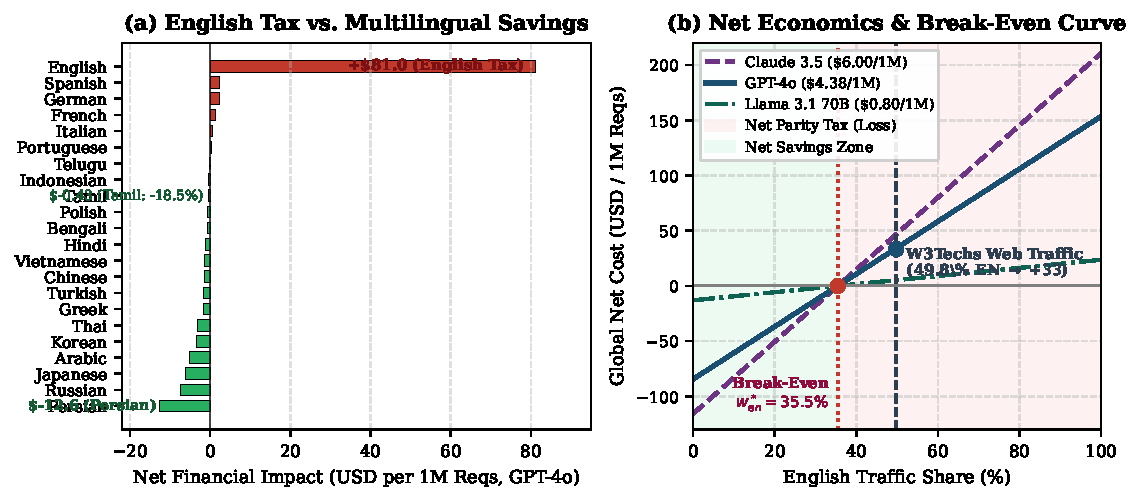
\includegraphics[width=\columnwidth]{figures/fig3_cost_simulation.pdf}
    \vspace{-1.4em}
    \caption{Global financial impact across 1M requests. (a) English Tax ($+\$81.03$) dwarfs non-English savings ($-\$39.87$). (b) Break-even occurs at $w_{\mathrm{en}}^* = 35.5\%$; web ($50\%$) and enterprise ($75\%$) traffic operate in net financial penalty.}
    \label{fig:cost_simulation}
    \vspace{-0.6em}
\end{figure}

\textbf{The ``English Tax'' vs.\ Multilingual Savings:} Figure~\ref{fig:cost_simulation}(a) details the financial balance. PA-BPE inflates English token counts by $+8.51\%$ on FLORES-200 ($+35.1$ tokens/req). With English commanding $49.8\%$ of web content ($52.8\%$ normalized), this adds an ``English Tax'' of $\mathbf{+\$81.03}$ per 1M requests on GPT-4o ($+\$111.12$ on Claude 3.5). While Dravidian scripts save tokens (Tamil: $-18.5\%$; Telugu: $-17.2\%$), their minuscule web share (Tamil: $0.05\%$) caps total savings across all 21 non-English languages at only $\mathbf{-\$39.87}$. The global net balance is a financial loss of $\mathbf{+\$41.16}$ per 1M requests on GPT-4o ($\mathbf{+\$56.43}$ on Claude 3.5; $\mathbf{+\$41,160.00}$ annually per billion requests).

\textbf{Break-Even Traffic Dynamics:} In Figure~\ref{fig:cost_simulation}(b), the analytical break-even point occurs at:
\begin{equation}
w_{\mathrm{en}}^* = \frac{-\overline{\Delta T}_{\mathrm{non\text{-}en}}}{\Delta T_{\mathrm{en}} - \overline{\Delta T}_{\mathrm{non\text{-}en}}} = \frac{-(-19.30)}{35.10 - (-19.30)} = \mathbf{35.48\%}.
\label{eq:breakeven}
\end{equation}
Because web ($50\%$) and enterprise software ($70\%$--$80\%$) exceed $35.5\%$, PA-BPE operates permanently inside the net surcharge zone.
